\PassOptionsToPackage{unicode=true}{hyperref} % options for packages loaded elsewhere
\PassOptionsToPackage{hyphens}{url}
%
\documentclass[]{article}
\usepackage{lmodern}
\usepackage{amssymb,amsmath}
\usepackage{ifxetex,ifluatex}
\usepackage{fixltx2e} % provides \textsubscript
\ifnum 0\ifxetex 1\fi\ifluatex 1\fi=0 % if pdftex
  \usepackage[T1]{fontenc}
  \usepackage[utf8]{inputenc}
  \usepackage{textcomp} % provides euro and other symbols
\else % if luatex or xelatex
  \usepackage{unicode-math}
  \defaultfontfeatures{Ligatures=TeX,Scale=MatchLowercase}
\fi
% use upquote if available, for straight quotes in verbatim environments
\IfFileExists{upquote.sty}{\usepackage{upquote}}{}
% use microtype if available
\IfFileExists{microtype.sty}{%
\usepackage[]{microtype}
\UseMicrotypeSet[protrusion]{basicmath} % disable protrusion for tt fonts
}{}
\IfFileExists{parskip.sty}{%
\usepackage{parskip}
}{% else
\setlength{\parindent}{0pt}
\setlength{\parskip}{6pt plus 2pt minus 1pt}
}
\usepackage{hyperref}
\hypersetup{
            pdftitle={Wine Quality},
            pdfauthor={Alexandre SALMON, Thomas FRION},
            pdfborder={0 0 0},
            breaklinks=true}
\urlstyle{same}  % don't use monospace font for urls
\usepackage[margin=1in]{geometry}
\usepackage{color}
\usepackage{fancyvrb}
\newcommand{\VerbBar}{|}
\newcommand{\VERB}{\Verb[commandchars=\\\{\}]}
\DefineVerbatimEnvironment{Highlighting}{Verbatim}{commandchars=\\\{\}}
% Add ',fontsize=\small' for more characters per line
\usepackage{framed}
\definecolor{shadecolor}{RGB}{248,248,248}
\newenvironment{Shaded}{\begin{snugshade}}{\end{snugshade}}
\newcommand{\AlertTok}[1]{\textcolor[rgb]{0.94,0.16,0.16}{#1}}
\newcommand{\AnnotationTok}[1]{\textcolor[rgb]{0.56,0.35,0.01}{\textbf{\textit{#1}}}}
\newcommand{\AttributeTok}[1]{\textcolor[rgb]{0.77,0.63,0.00}{#1}}
\newcommand{\BaseNTok}[1]{\textcolor[rgb]{0.00,0.00,0.81}{#1}}
\newcommand{\BuiltInTok}[1]{#1}
\newcommand{\CharTok}[1]{\textcolor[rgb]{0.31,0.60,0.02}{#1}}
\newcommand{\CommentTok}[1]{\textcolor[rgb]{0.56,0.35,0.01}{\textit{#1}}}
\newcommand{\CommentVarTok}[1]{\textcolor[rgb]{0.56,0.35,0.01}{\textbf{\textit{#1}}}}
\newcommand{\ConstantTok}[1]{\textcolor[rgb]{0.00,0.00,0.00}{#1}}
\newcommand{\ControlFlowTok}[1]{\textcolor[rgb]{0.13,0.29,0.53}{\textbf{#1}}}
\newcommand{\DataTypeTok}[1]{\textcolor[rgb]{0.13,0.29,0.53}{#1}}
\newcommand{\DecValTok}[1]{\textcolor[rgb]{0.00,0.00,0.81}{#1}}
\newcommand{\DocumentationTok}[1]{\textcolor[rgb]{0.56,0.35,0.01}{\textbf{\textit{#1}}}}
\newcommand{\ErrorTok}[1]{\textcolor[rgb]{0.64,0.00,0.00}{\textbf{#1}}}
\newcommand{\ExtensionTok}[1]{#1}
\newcommand{\FloatTok}[1]{\textcolor[rgb]{0.00,0.00,0.81}{#1}}
\newcommand{\FunctionTok}[1]{\textcolor[rgb]{0.00,0.00,0.00}{#1}}
\newcommand{\ImportTok}[1]{#1}
\newcommand{\InformationTok}[1]{\textcolor[rgb]{0.56,0.35,0.01}{\textbf{\textit{#1}}}}
\newcommand{\KeywordTok}[1]{\textcolor[rgb]{0.13,0.29,0.53}{\textbf{#1}}}
\newcommand{\NormalTok}[1]{#1}
\newcommand{\OperatorTok}[1]{\textcolor[rgb]{0.81,0.36,0.00}{\textbf{#1}}}
\newcommand{\OtherTok}[1]{\textcolor[rgb]{0.56,0.35,0.01}{#1}}
\newcommand{\PreprocessorTok}[1]{\textcolor[rgb]{0.56,0.35,0.01}{\textit{#1}}}
\newcommand{\RegionMarkerTok}[1]{#1}
\newcommand{\SpecialCharTok}[1]{\textcolor[rgb]{0.00,0.00,0.00}{#1}}
\newcommand{\SpecialStringTok}[1]{\textcolor[rgb]{0.31,0.60,0.02}{#1}}
\newcommand{\StringTok}[1]{\textcolor[rgb]{0.31,0.60,0.02}{#1}}
\newcommand{\VariableTok}[1]{\textcolor[rgb]{0.00,0.00,0.00}{#1}}
\newcommand{\VerbatimStringTok}[1]{\textcolor[rgb]{0.31,0.60,0.02}{#1}}
\newcommand{\WarningTok}[1]{\textcolor[rgb]{0.56,0.35,0.01}{\textbf{\textit{#1}}}}
\usepackage{graphicx,grffile}
\makeatletter
\def\maxwidth{\ifdim\Gin@nat@width>\linewidth\linewidth\else\Gin@nat@width\fi}
\def\maxheight{\ifdim\Gin@nat@height>\textheight\textheight\else\Gin@nat@height\fi}
\makeatother
% Scale images if necessary, so that they will not overflow the page
% margins by default, and it is still possible to overwrite the defaults
% using explicit options in \includegraphics[width, height, ...]{}
\setkeys{Gin}{width=\maxwidth,height=\maxheight,keepaspectratio}
\setlength{\emergencystretch}{3em}  % prevent overfull lines
\providecommand{\tightlist}{%
  \setlength{\itemsep}{0pt}\setlength{\parskip}{0pt}}
\setcounter{secnumdepth}{0}
% Redefines (sub)paragraphs to behave more like sections
\ifx\paragraph\undefined\else
\let\oldparagraph\paragraph
\renewcommand{\paragraph}[1]{\oldparagraph{#1}\mbox{}}
\fi
\ifx\subparagraph\undefined\else
\let\oldsubparagraph\subparagraph
\renewcommand{\subparagraph}[1]{\oldsubparagraph{#1}\mbox{}}
\fi

% set default figure placement to htbp
\makeatletter
\def\fps@figure{htbp}
\makeatother


\title{Wine Quality}
\author{Alexandre SALMON, Thomas FRION}
\date{13/01/2021}

\begin{document}
\maketitle

\hypertarget{objectif-de-luxe9tude}{%
\section{1 Objectif de l'étude}\label{objectif-de-luxe9tude}}

Notre étude va porter sur la qualité des vins portugais, de la région
Vinho Verde. Nos objectifs via cette étude sont :

\begin{itemize}
\tightlist
\item
  Déterminer un modèle de prédiction de la qualité d'un vin rouge et
  d'un vin blanc. Ainsi, connaitre le critère physionomique le plus
  important dans la détermination de la qualité pour chaque type de vin.
\item
  Comparer les deux modèles (blanc et rouge) pour savoir si ce qui vait
  un bon vin blanc, fait un bon vin rouge
\end{itemize}

Les conclusions de cette étude pourront permettre aux vignerons
d'améliorer la qualité de leurs vins.

\hypertarget{analyse-descriptive}{%
\section{2 Analyse descriptive}\label{analyse-descriptive}}

Pour cette étude nous disposons de deux jeux de données : un pour le vin
rouge et 1 pour le vin blanc. Nous avons obtenu ces données sur la page
\href{https://archive.ics.uci.edu/ml/datasets/Wine+Quality}{UCI: Wine
Quality Data Set}

Pour les deux jeux de données nous avons douze variables: onze variables
d'entrée qui correspondent aux critères physionomiques du vin et une
variable de sortie qui correspond à la qualité du vin en 0 et 10. Les
onze critères physionomiques sont les suivantes :

\begin{enumerate}
\def\labelenumi{\arabic{enumi}.}
\tightlist
\item
  Acidité fixe (ou acidité naturelle du raisin)
\item
  Acidité volatile (teneur d'acides gras)
\item
  Acide citrique (teneur d'acide citrique)
\item
  Sucre résiduel (sucres encore présents après la fermentation)
\item
  Chlorures (teneur des différents chlorures)
\item
  Dioxyde de soufre (\(SO_2\)) libre (teneur du principe actif du
  \(SO_2\))
\item
  Total du dioxyde de soufre (\(SO_2\)) (teneur de toutes les formes du
  \(SO_2\))
\item
  Densité
\item
  pH
\item
  Sulfates (teneur du fongicide)
\item
  Alcool
\end{enumerate}

La variable de sortie correspond à la médianne des notes données par des
experts (au minimun trois notes). Si la variable vaut 0 sela signifie
que le vin est de très mauvaise qualité. Si la variable vaut 10 alors le
vin est de bonne qualité.

Nous avons 1599 vins rouges et 4898 vins blancs.

\begin{Shaded}
\begin{Highlighting}[]
\NormalTok{RWine <-}\StringTok{ }\KeywordTok{read.csv}\NormalTok{(}\StringTok{"./data/winequality-red.csv"}\NormalTok{, }\DataTypeTok{sep =} \StringTok{";"}\NormalTok{); }
\NormalTok{WWine <-}\StringTok{ }\KeywordTok{read.csv}\NormalTok{(}\StringTok{"./data/winequality-white.csv"}\NormalTok{, }\DataTypeTok{sep =} \StringTok{";"}\NormalTok{);}
\end{Highlighting}
\end{Shaded}

Afin de connaître les liens entre les variables d'entrée, nous avons
décidé de calculer la corrélation entre les différentes variables. Ce
calcul nous a données les résultats suivants :

\begin{Shaded}
\begin{Highlighting}[]
\NormalTok{WWine[}\StringTok{'type'}\NormalTok{]=}\StringTok{'White'}
\NormalTok{RWine[}\StringTok{'type'}\NormalTok{]=}\StringTok{'Red'}
\NormalTok{AWine<-}\KeywordTok{rbind}\NormalTok{(RWine, WWine)}
\NormalTok{AWine.m <-}\StringTok{ }\KeywordTok{melt}\NormalTok{(AWine, }\DataTypeTok{id.var =} \StringTok{"type"}\NormalTok{)}

\KeywordTok{ggcorr}\NormalTok{(AWine[, }\DecValTok{-1}\NormalTok{], }\DataTypeTok{geom =} \StringTok{"blank"}\NormalTok{, }\DataTypeTok{label =} \OtherTok{TRUE}\NormalTok{, }\DataTypeTok{hjust =} \FloatTok{0.75}\NormalTok{) }\OperatorTok{+}
\StringTok{  }\KeywordTok{geom_point}\NormalTok{(}\DataTypeTok{size =} \DecValTok{10}\NormalTok{, }\KeywordTok{aes}\NormalTok{(}\DataTypeTok{color =}\NormalTok{ coefficient }\OperatorTok{>}\StringTok{ }\DecValTok{0}\NormalTok{, }\DataTypeTok{alpha =} \KeywordTok{abs}\NormalTok{(coefficient) }\OperatorTok{>}\StringTok{ }\FloatTok{0.5}\NormalTok{)) }\OperatorTok{+}
\StringTok{  }\KeywordTok{scale_alpha_manual}\NormalTok{(}\DataTypeTok{values =} \KeywordTok{c}\NormalTok{(}\StringTok{"TRUE"}\NormalTok{ =}\StringTok{ }\FloatTok{0.25}\NormalTok{, }\StringTok{"FALSE"}\NormalTok{ =}\StringTok{ }\DecValTok{0}\NormalTok{)) }\OperatorTok{+}
\StringTok{  }\KeywordTok{guides}\NormalTok{(}\DataTypeTok{color =} \OtherTok{FALSE}\NormalTok{, }\DataTypeTok{alpha =} \OtherTok{FALSE}\NormalTok{)}
\end{Highlighting}
\end{Shaded}

\begin{verbatim}
## Warning in ggcorr(AWine[, -1], geom = "blank", label = TRUE, hjust = 0.75): data
## in column(s) 'type' are not numeric and were ignored
\end{verbatim}

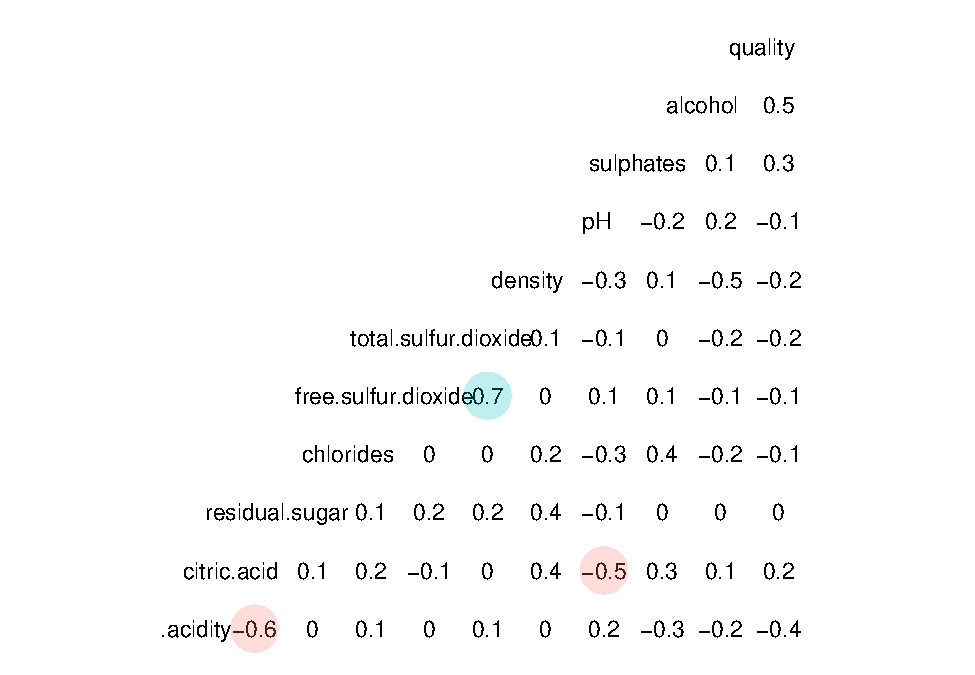
\includegraphics{repport_files/figure-latex/unnamed-chunk-2-1.pdf}

Nous pouvons observer dans les résultats ci-desssus, qu'il y a des
corrélations positives et négatives. Par exemple, la densité et l'alcool
ont une corrélation négative : cela signifie que plus il y a d'alcool
moins le vin est dense. À l'inverse, le \(SO_2\) libre et le \(SO_2\)
total ont une corrélation positive. Ce qui signifie que plus il y a de
\(SO_2\) libre plus la teneur totale de \(SO_2\) sera importante.

Nous avons choisis de faire le calcul des corrélations afin d'avoir une
vision d'ensemble des liens entre les variables. Ainsi nous pouvons
faire un plot plus lisible des données pour mieux apprécier les liens.

Nous pouvons déjà annoncer un lien entre deux variables : \(SO_2\) libre
et \(SO_2\) total. Ce lien est le suivant :

\begin{Shaded}
\begin{Highlighting}[]
\KeywordTok{plot}\NormalTok{(AWine[}\DecValTok{1}\OperatorTok{:}\DecValTok{100}\NormalTok{,}\KeywordTok{c}\NormalTok{(}\DecValTok{1}\NormalTok{,}\DecValTok{2}\NormalTok{,}\DecValTok{3}\NormalTok{,}\DecValTok{6}\NormalTok{,}\DecValTok{7}\NormalTok{,}\DecValTok{8}\NormalTok{,}\DecValTok{9}\NormalTok{)])}
\end{Highlighting}
\end{Shaded}

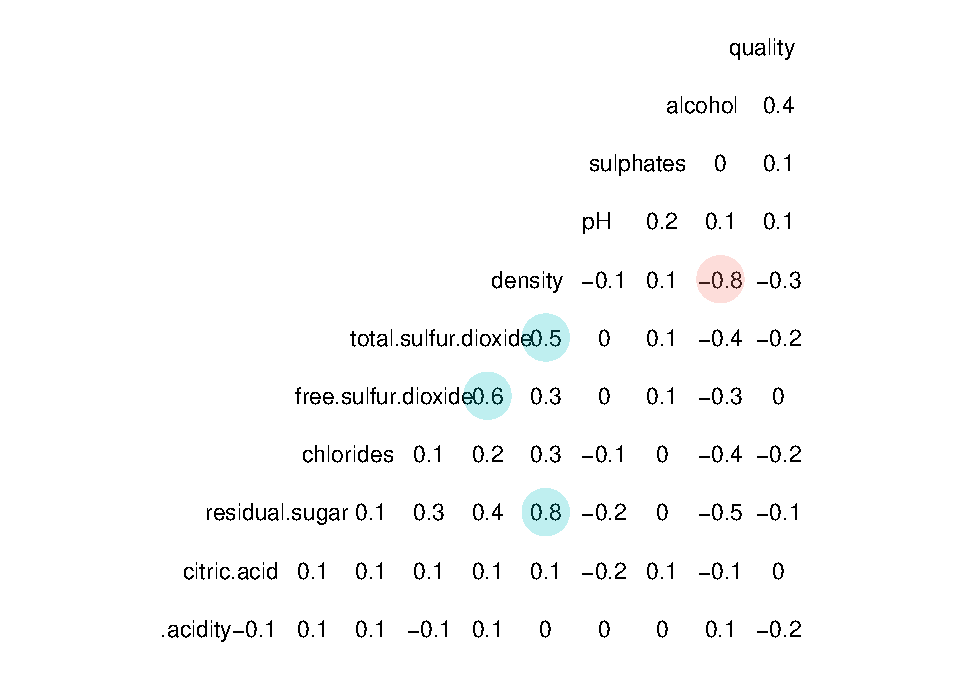
\includegraphics{repport_files/figure-latex/unnamed-chunk-3-1.pdf}

\begin{Shaded}
\begin{Highlighting}[]
\NormalTok{AWine}\OperatorTok{$}\NormalTok{type<-}\OtherTok{NULL}

\NormalTok{arr =}\StringTok{ }\KeywordTok{c}\NormalTok{()}
\ControlFlowTok{for}\NormalTok{ (i }\ControlFlowTok{in} \DecValTok{2}\OperatorTok{:}\DecValTok{15}\NormalTok{) \{}
\NormalTok{  res <-}\StringTok{ }\KeywordTok{kmeans}\NormalTok{(AWine,i)}
\NormalTok{  arr<-}\KeywordTok{c}\NormalTok{(arr,res}\OperatorTok{$}\NormalTok{tot.withinss}\OperatorTok{/}\NormalTok{res}\OperatorTok{$}\NormalTok{totss)}
\NormalTok{\}}
\end{Highlighting}
\end{Shaded}

\begin{verbatim}
## Warning: did not converge in 10 iterations
\end{verbatim}

\begin{Shaded}
\begin{Highlighting}[]
\KeywordTok{plot}\NormalTok{(arr)}
\end{Highlighting}
\end{Shaded}

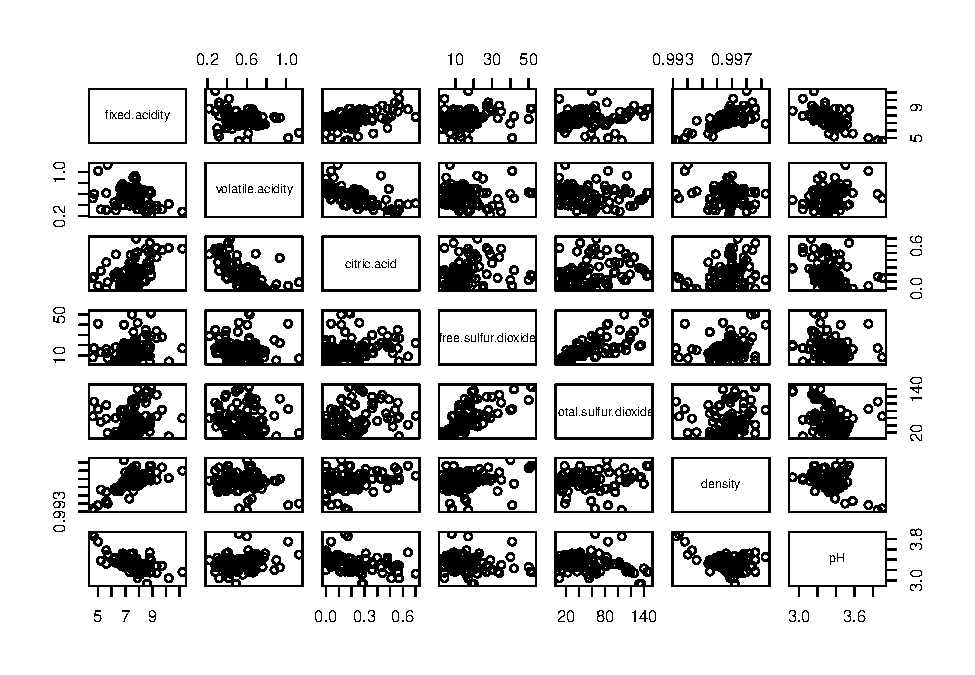
\includegraphics{repport_files/figure-latex/unnamed-chunk-4-1.pdf}

\end{document}
